\subsection{Kvalitetsscenarier}
Safety/sikkerhed: \\
Brugeren: Kan brugeren komme til skade \\

Security/sikkerhed: \\
Systemet: Kan systemet �del�gges \\
Brugeren: Er brugerens data sikret. \\

Reliability/p�lidelighed: \\
Systemet: Er systemet stabilt. \\
Appen: Kan brugeren stole p� informationen. \\

Resilience/modstandsdygtigt: \\
Systemet: Kan komme op at k�re hurtigt igen efter problemer. \\

Robustness/robust: \\
Systemet: Stabilt og crasher ikke. \\
Database: Kan h�ndtere foresp�rgsler. \\

Testability/testbart: \\
App: Funktionaliteten er testbar som sikrer usability. \\

Adaptability/tilpasseligt: \\
Systemet: Kan tilpasses i forhold til udvikling af nyt system eller kravs�ndringer. \\

Modularity/modul�rt:\\ 
Systemet: N�dvendighed for adaptability og scalability.\\

Complexity/komplekst: \\
Systemet: FoodMap kompleksitet, algoritme. Modvirker adaptability? \\

Portability/overf�rlighed:\\ 
App: Kan portes til andre platforme. \\


Usability/brugbarhed: \\
App: Nemt at bruge. Vigtigt \\

Reusability/genbrugelighed: \\
App: videre udvikling, diabetiker, fitness app. \\
Database: genbrug til anden platform. \\


Vigtige: \\
- Resilience: **** \\
- Testability: ***** \\
- Adaptability: **** \\
- Modularity: **** \\
- Compleksitet: *** \\
- Portability: ** \\
- Usability: ***** \\
- Reusability: *

\subsection{Kravscenerier}
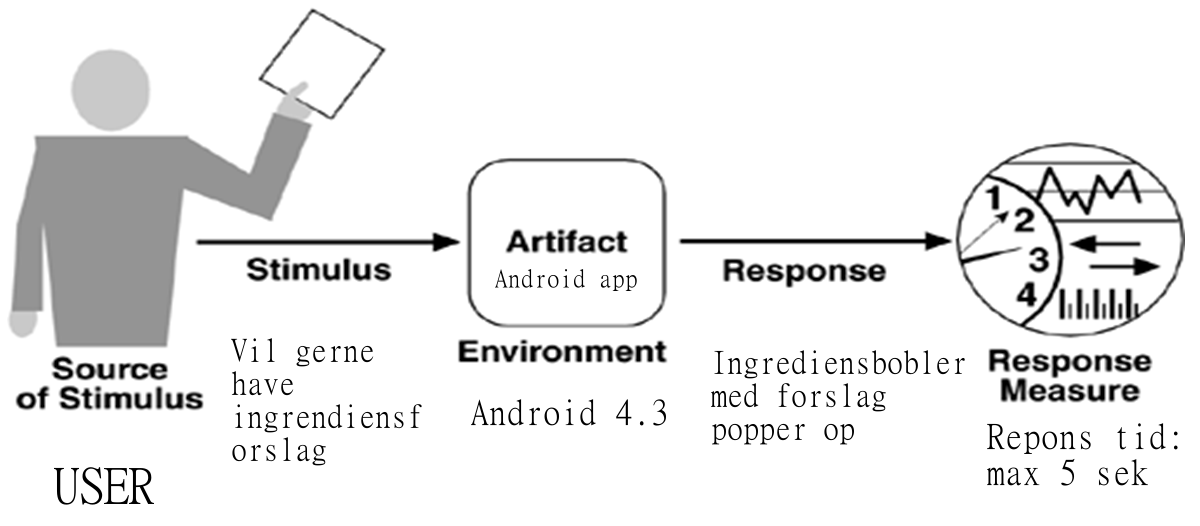
\includegraphics[scale=0.30]{includes/billeder/kravsscenerie_foodwheel.png} \\

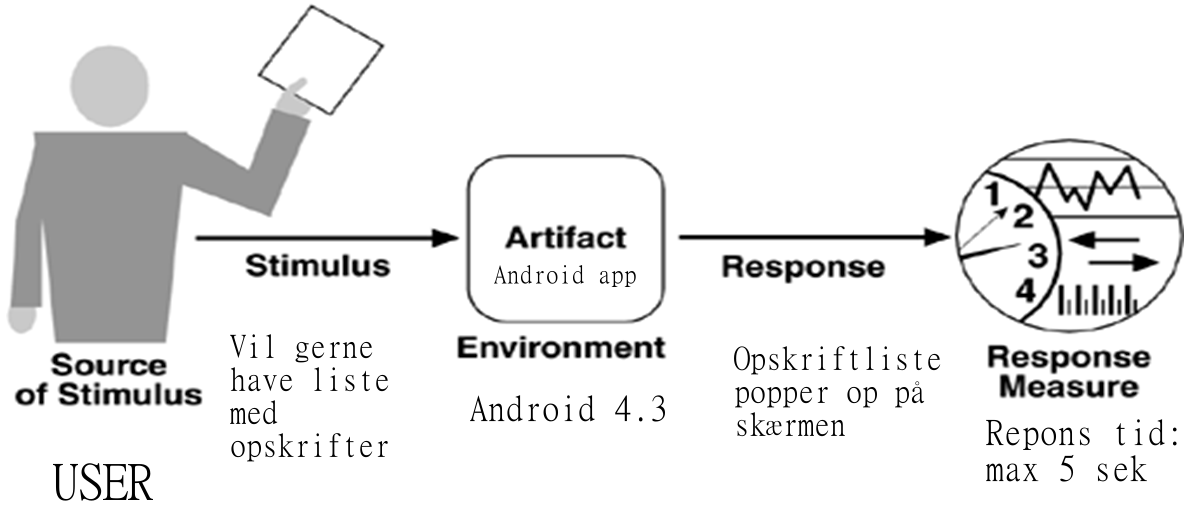
\includegraphics[scale=0.30]{includes/billeder/kravsscenerie_opskriftliste.png}